% \chapter{The first appendix}

% Text for the first appendix goes here.

% \section{Appendix section}

% Text for a section in the first appendix goes here.

% test ทดสอบฟอนต์ serif

% \textsf{test ทดสอบฟอนต์ sans serif}

\ifenglish\else
% TODO: Thai teletype font still doesn't work with english option
% \verb+test ทดสอบฟอนต์ teletype ภาษาไทย+

% \texttt{test ทดสอบฟอนต์ teletype ภาษาไทย}
\fi

\chapter{\ifenglish Manual\else คู่มือการใช้งานระบบ\fi}
แอพพลิเคชันรองรับการทำงานบนระบบปฏิบัติการ Ubuntu หรือ Ubuntu based ซึ่งต้องมีการติดตั้งโปรแกรมดังต่อไปนี้
\begin{enumerate}
  \item Docker
  \item Yarn
  \item Terraform
\end{enumerate}

\section{คู่มือการติดตั้งโปรแกรมที่จำเป็นในการติดตั้งแอพพลิเคชัน}
\subsection{การติดตั้ง Docker}
\begin{enumerate}
  \item เปิด Terminal ของ Ubuntu
  \item ลบ packages ที่เกี่ยวกับ docker ด้วยคำสั่ง 
  \begin{verbatim}
    sudo apt-get remove docker docker-engine docker.io containerd runc
  \end{verbatim}
  \item อัพเดท apt-get ต่างๆด้วยคำสั่ง 
  \begin{verbatim}
    sudo apt-get update
  \end{verbatim}
  \item ติดตั้ง packages สำหรับการดึงข้อมูลผ่านด้วยคำสั่ง 
  \begin{verbatim}
    sudo apt-get install ca-certificates curl gnupg
  \end{verbatim}
  \item สร้างไดเรกทอรีสำหรับเก็บ Docker GPG Key ด้วยคำสั่ง 
  \begin{verbatim}
    sudo mkdir -m 0755 -p /etc/apt/keyrings
  \end{verbatim}
  \item เพิ่ม Docker GPG Key ด้วย 
  \begin{verbatim}
    curl -fsSL https://download.docker.com/linux/ubuntu/gpg | \
    sudo gpg --dearmor -o /etc/apt/keyrings/docker.gpg
  \end{verbatim}
  \item เพิ่ม Docker repository ไปใน apt ด้วยคำสั่ง 
  \begin{verbatim}
    echo \
  "deb [arch="$(dpkg --print-architecture)" signed-by=/etc/apt/keyrings/docker.gpg] \
  https://download.docker.com/linux/ubuntu \
  "$(. /etc/os-release && echo "$VERSION_CODENAME")" stable" | \
  sudo tee /etc/apt/sources.list.d/docker.list > /dev/null
  \end{verbatim}
  \item อัพเดท Docker repository ด้วยคำสั่ง 
  \begin{verbatim}
    sudo apt-get update
  \end{verbatim}
  \item ติดตั้ง Docker ผ่าน apt ด้วยคำสั่ง 
  \begin{verbatim}
    sudo apt-get install \
    docker-ce \
    docker-ce-cli \
    containerd.io \
    docker-buildx-plugin \
    docker-compose-plugin
  \end{verbatim}
  \item สร้าง user group docker ด้วยคำสั่ง 
  \begin{verbatim}
    sudo groupadd docker
  \end{verbatim}
  \item เพิ่ม user ปัจจุบันใน docker group ด้วยคำสั่ง 
  \begin{verbatim}
    sudo usermod -aG docker $User
  \end{verbatim}
  \item ทำการเปิดใช้งาน docker group ด้วยคำสั่ง 
  \begin{verbatim}
    newgrp docker
  \end{verbatim}
\end{enumerate} 
หรือสามารถศึกษาเพิ่มเติมได้ที่ \href
{https://docs.docker.com/engine/install/ubuntu/}
{คู่มือการติดตั้ง Docker}
%
\subsection{การติดตั้ง Yarn}
\begin{enumerate}
  \item เปิด Terminal ของ Ubuntu
  \item เพิ่ม GPG Key และ Yarn repository ด้วยคำสั่ง 
  \begin{verbatim}
    echo "deb https://dl.yarnpkg.com/debian/ stable main" | \
    sudo tee /etc/apt/sources.list.d/yarn.list
  \end{verbatim}
  \item อัพเดท Yarn repository ด้วยคำสั่ง 
  \begin{verbatim}
    sudo apt-get update
  \end{verbatim}
  \item ติดตั้ง Yarn ผ่าน apt ด้วยคำสั่ง 
  \begin{verbatim}
    sudo apt install yarn
  \end{verbatim}
  \item ตรวจสอบเวอร์ชันของ Yarn ด้วยคำสั่ง 
  \begin{verbatim}
    yarn --version
  \end{verbatim}
\end{enumerate}
หรือสามารถศึกษาเพิ่มเติมได้ที่ \href
{https://linuxize.com/post/how-to-install-yarn-on-ubuntu-20-04/}
{คู่มือการติดตั้ง Yarn}
%
\subsection{การติดตั้ง Terraform}
\begin{enumerate}
  \item เปิด Terminal ของ Ubuntu
  \item เตรียม packages ในการเพิ่ม GPG Key ด้วยคำสั่ง 
  \begin{verbatim}
    sudo apt-get update && \
    sudo apt-get install -y \
      gnupg software-properties-common
  \end{verbatim}
  \item เพิ่ม Hashicorp GPG Key ด้วยคำสั่ง
  \begin{verbatim}
    wget -O- https://apt.releases.hashicorp.com/gpg | \
    gpg --dearmor | \
    sudo tee /usr/share/keyrings/hashicorp-archive-keyring.gpg
  \end{verbatim}
  \item ตรวจสอบ GPG KEY ด้วยคำสั่ง 
  \begin{verbatim}
    gpg --no-default-keyring \
    --keyring /usr/share/keyrings/hashicorp-archive-keyring.gpg \
    --fingerprint
  \end{verbatim}
  \item เพิ่ม Hashicorp repository ด้วยคำสั่ง 
  \begin{verbatim}
    echo "deb [signed-by=/usr/share/keyrings/hashicorp-archive-keyring.gpg] \
    https://apt.releases.hashicorp.com $(lsb_release -cs) main" | \
    sudo tee /etc/apt/sources.list.d/hashicorp.list
  \end{verbatim}
  \item อัพเดท Hashicorp repository ด้วยคำสั่ง 
  \begin{verbatim}
    sudo apt update
  \end{verbatim}
  \item ติดตั้ง Terraform ผ่าน apt ด้วยคำสั่ง 
  \begin{verbatim}
    sudo apt-get install terraform
  \end{verbatim}
\end{enumerate}
หรือสามารถศึกษาเพิ่มเติมได้ที่ \href
{https://developer.hashicorp.com/terraform/tutorials/aws-get-started/install-cli}
{คู่มือการติดตั้ง Terraform}
%
\section{คู่มือการติดตั้งแอพพลิเคชัน}
\begin{enumerate}
  \item เปิด Terminal ของ Ubuntu
  \item ทำการพิมพ์คำสั่ง 
  \begin{verbatim}
    git clone --depth 1 \
    https://github.com/Akaifox16/BestMatch.git \
    best-match
  \end{verbatim}
  \item เข้าไปในไดเรคทอรีของแอพพลิเคชันด้วยคำสั่ง 
  \begin{verbatim}
    cd best-match
  \end{verbatim}
  \item ใช้ text editor ที่สะดวกในการแก้ไขไฟล์ \path{terraform/postgres-manager/configs/host.tfvars}
  ชื่อ superuser (user) ของ PostgreSQL เป็น postgres และตั้งรหัสผ่าน (secret) ของ superuser ดังตัวอย่าง
  \begin{verbatim}
    connection = {
      host = "localhost"
      port = 5433
      user = "postgres"
      secret = "your password"
      sslmode = "disable"
    }
  \end{verbatim}
  \item เตรียมไฟล์ environment variables ด้วยคำสั่ง
  \begin{verbatim}
    cp .env.example .env && cp db.example.env db.env
  \end{verbatim}
  \item ใช้ text editor ที่สะดวกในการแก้ไขไฟล์ \path{./db.env} 
  ให้ POSTGRES\_PASSWORD เป็นรหัสผ่านเดียวกับใน \path{terraform/postgres-manager/configs/host.tfvars}
  \begin{verbatim}
    POSTGRES_PASSWORD="your password"
  \end{verbatim}
  \item ติดตั้งและรันแอพพลิเคชันด้วยคำสั่ง 
  \begin{verbatim}
    make
  \end{verbatim}
  หรือ
  \begin{verbatim}
    make install
  \end{verbatim}
\end{enumerate}
%
\section{คู่มือการใช้งานแอพพลิเคชัน}
เมื่อนักศึกษาเข้ามาที่เว็บแอพพลิเคชันจะพบกับหน้า Home
\begin{figure}[h]
  \begin{center}
    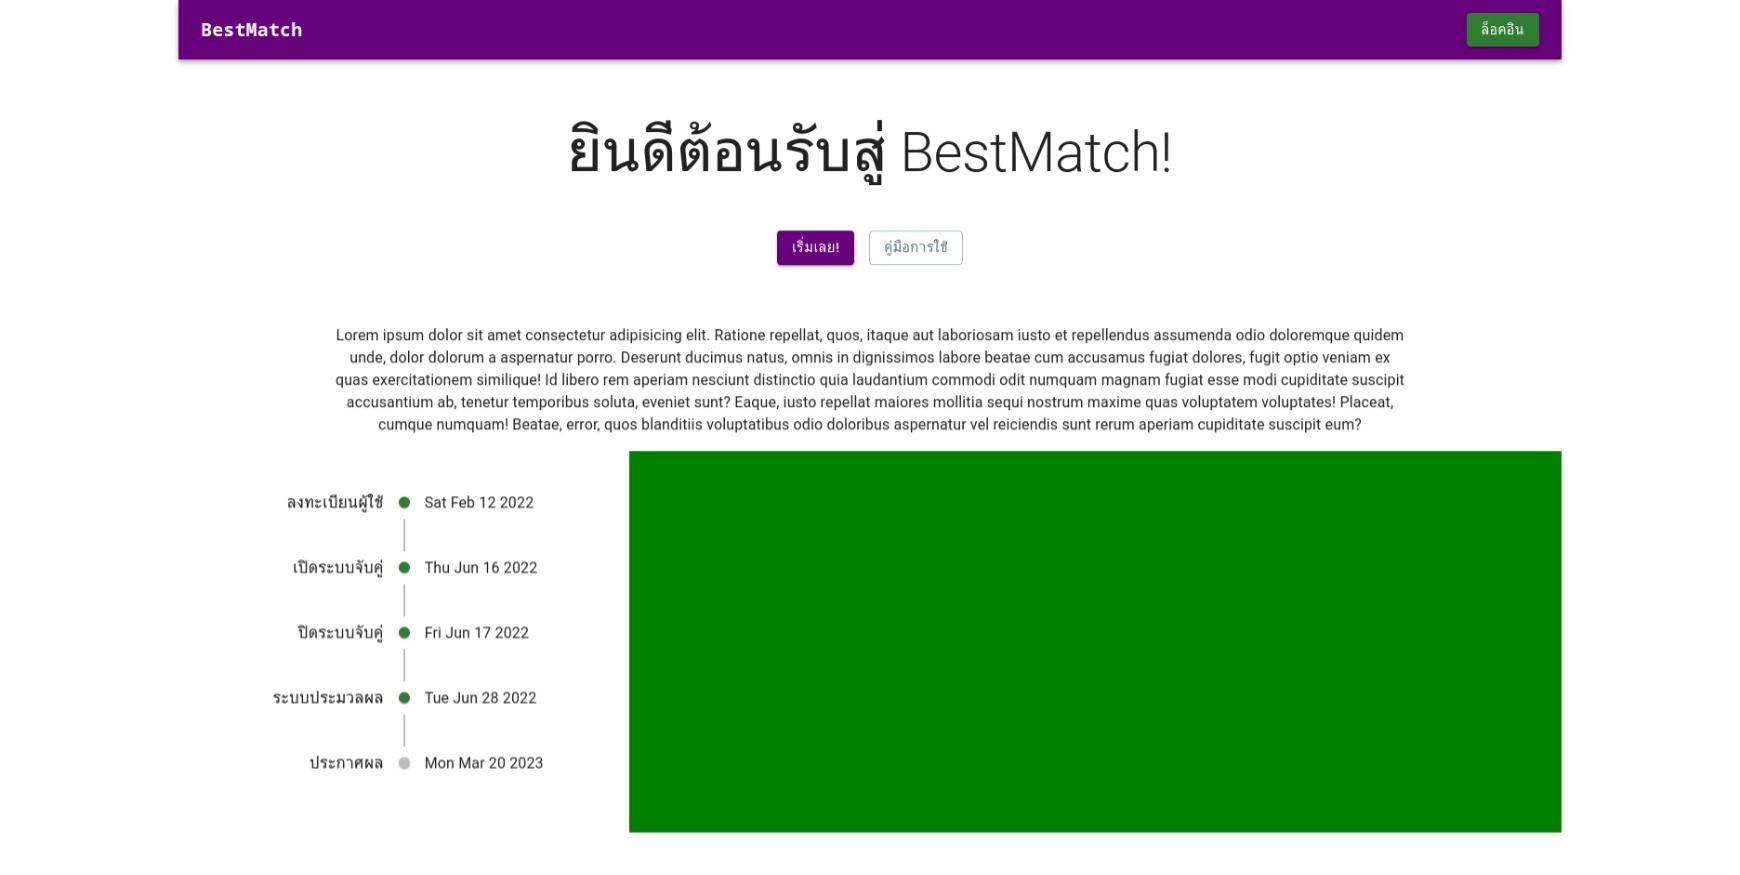
\includegraphics[width=\linewidth]{photo/web/student/home.jpeg}
  \end{center}
  \caption{หน้า Home}
\end{figure}
%
\newline
หลังจากนั้นจะกดปุ่ม "ล็อคอิน" หรือ "เริ่มเลย!" เพื่อทำการลงชื่อเข้าใช้
\begin{figure}[ht]
  \begin{center}
    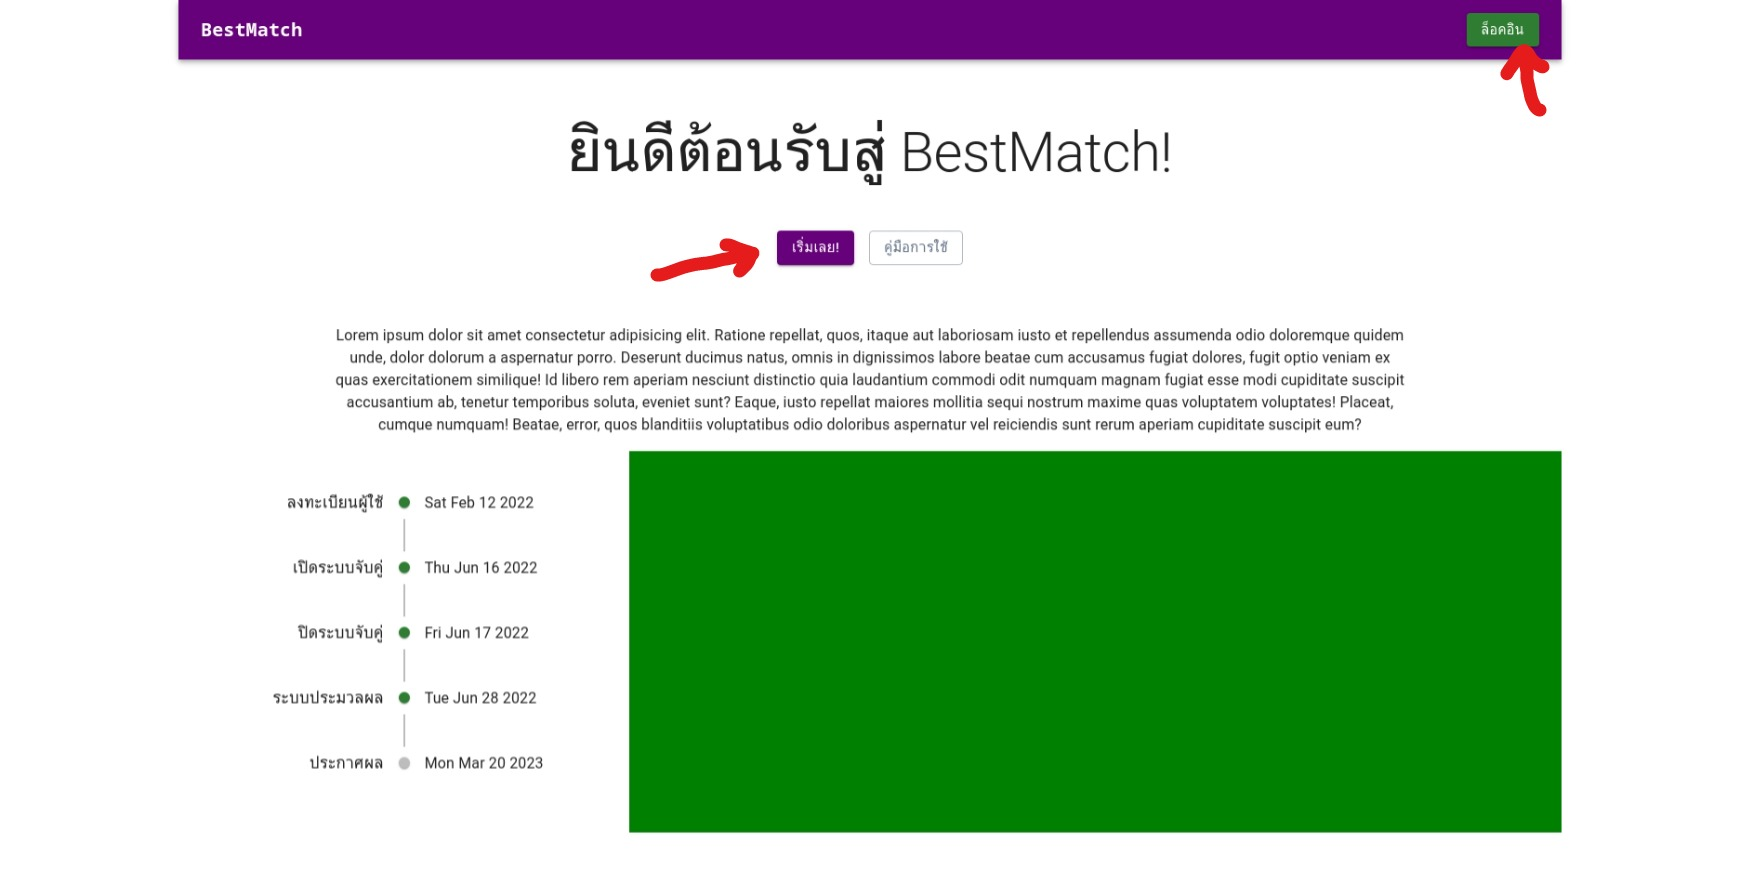
\includegraphics[width=\linewidth]{photo/web/student/login-btn.jpeg}
  \end{center}
  \caption{รูปตัวอย่างแสดงตำแหน่งปุ่ม "ล็อคอิน" และ "เริ่มเลย!"}
\end{figure}
\newpage 

หลังจากนั้นกรอกข้อมูลที่ใช้ในการยืนยันตัวตนในการเข้าใช้งาน
\begin{figure}[!ht]
  \begin{center}
    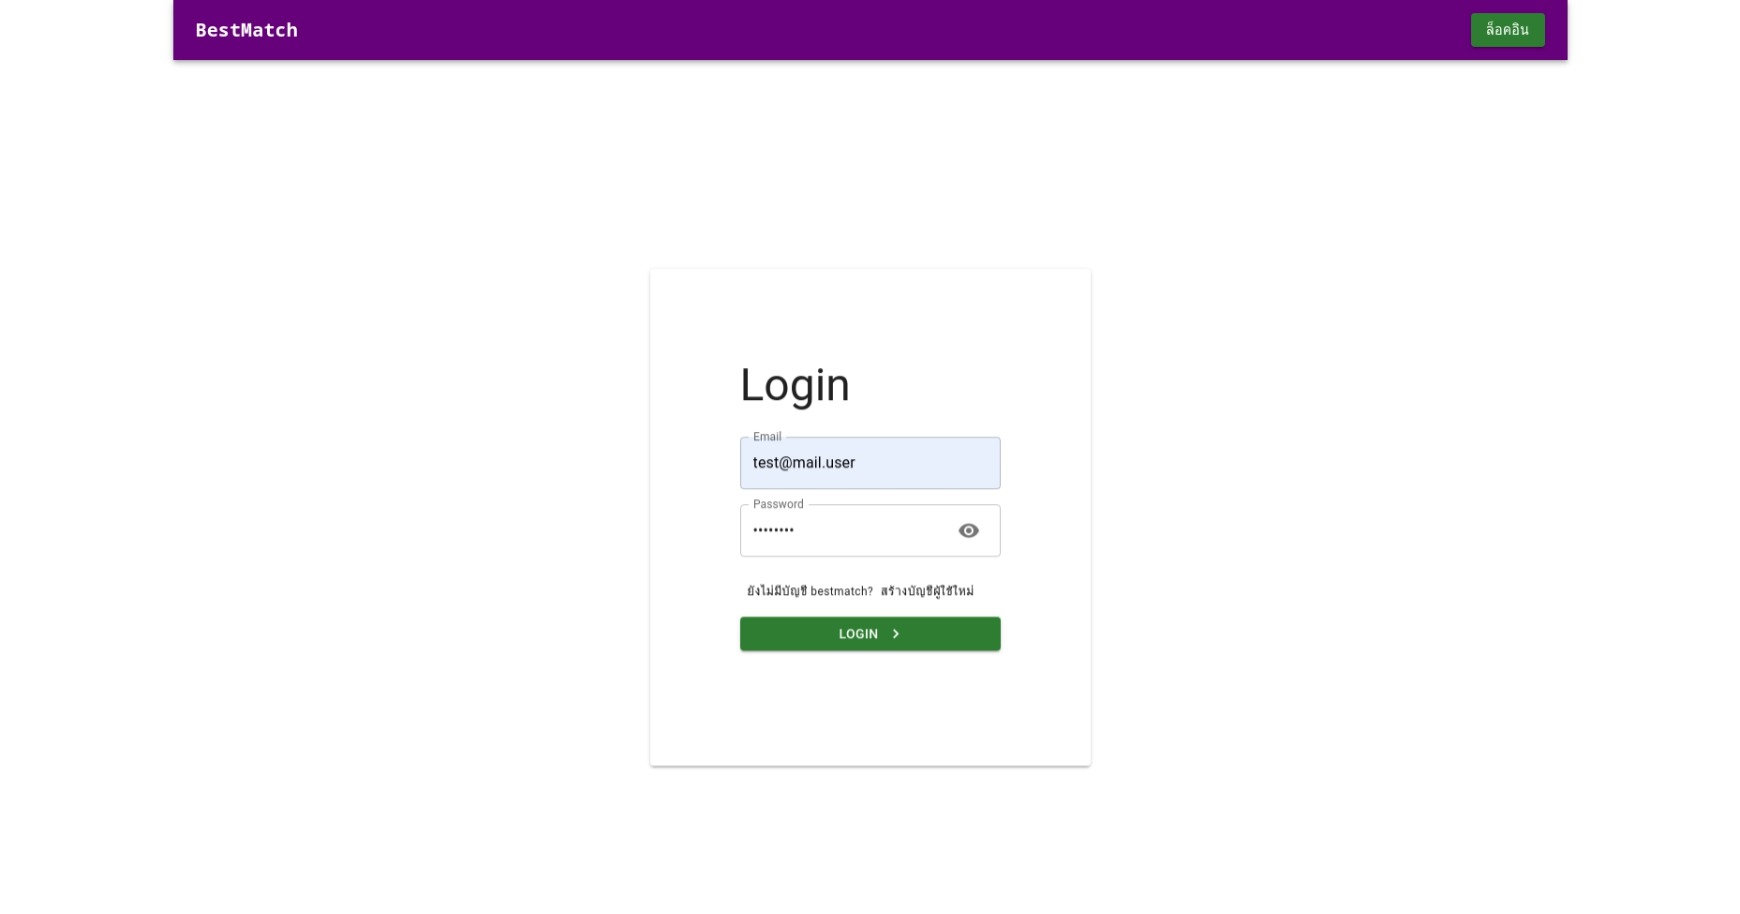
\includegraphics[width=\linewidth]{photo/web/student/login.jpeg}
  \end{center}
  \caption{หน้า Login}
\end{figure}
%
\newline
หากยังไม่มีบัญชีผู้ใช้จะต้องทำการสร้างบัญชีผู้ใช้โดยคลิกที่ "สร้างบัญชีผู้ใช้ใหม่"
\begin{figure}[!ht]
  \begin{center}
    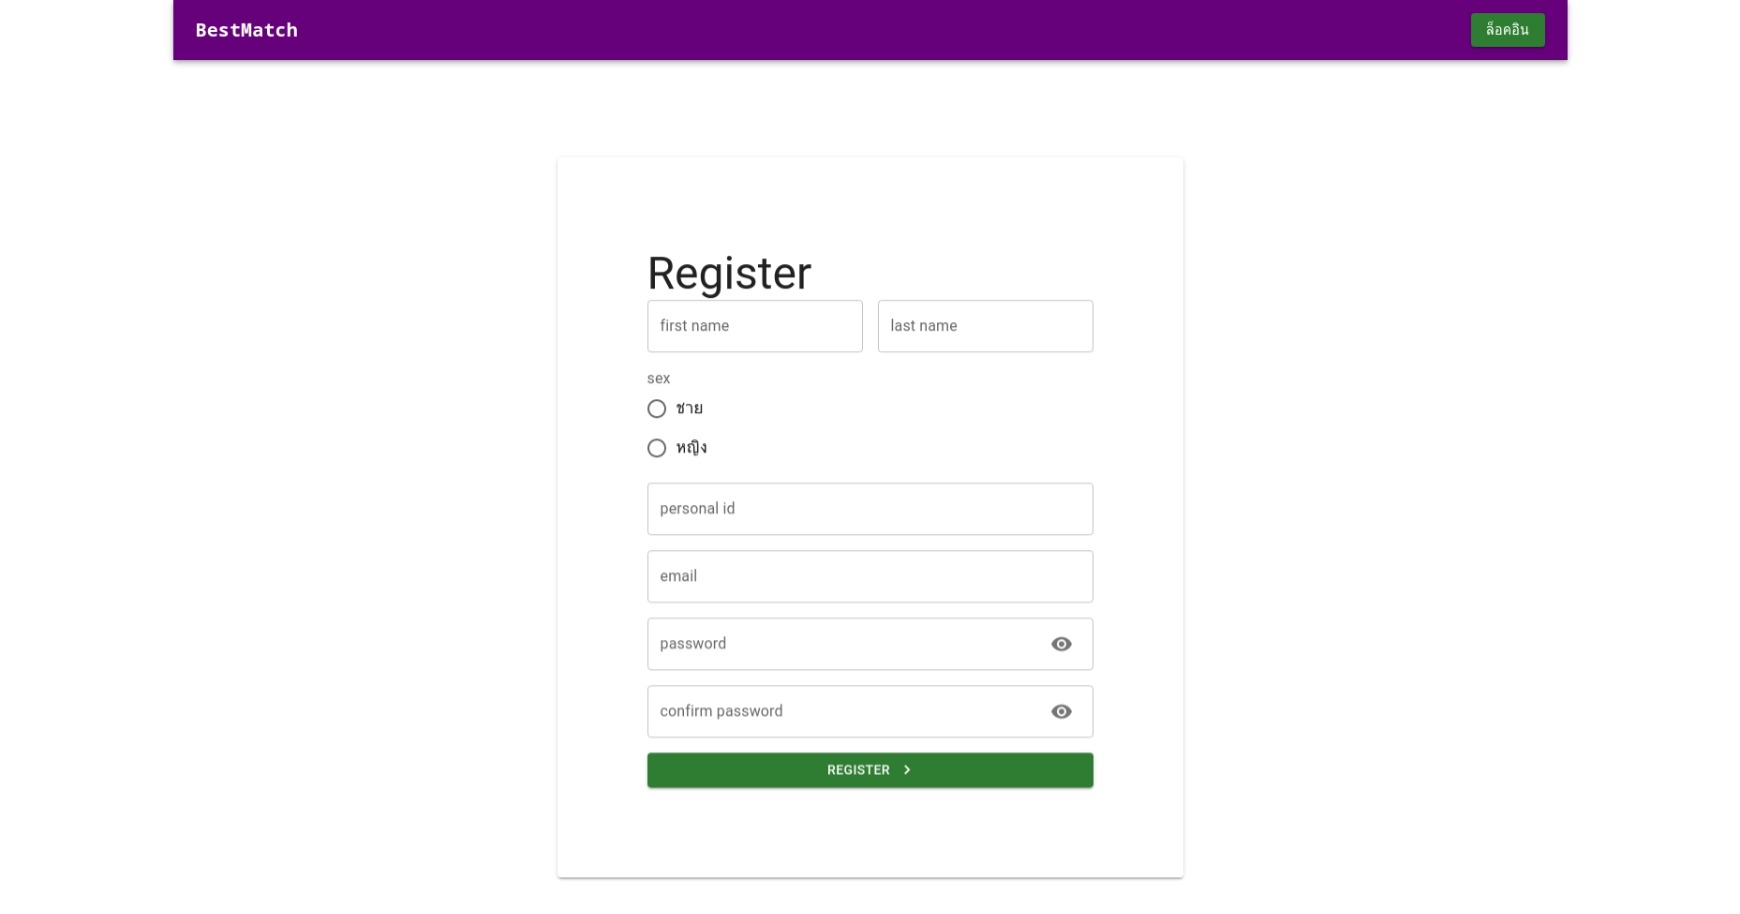
\includegraphics[width=\linewidth]{photo/web/student/register.jpeg}
  \end{center}
  \caption{หน้า Register}
\end{figure}
\newpage
%
เมื่อลงชื่อเข้าใช้แล้วจะกลับมาที่หน้า Home พร้อมกับอีเมล์ของผู้ใช้
\begin{figure}[!ht]
  \begin{center}
    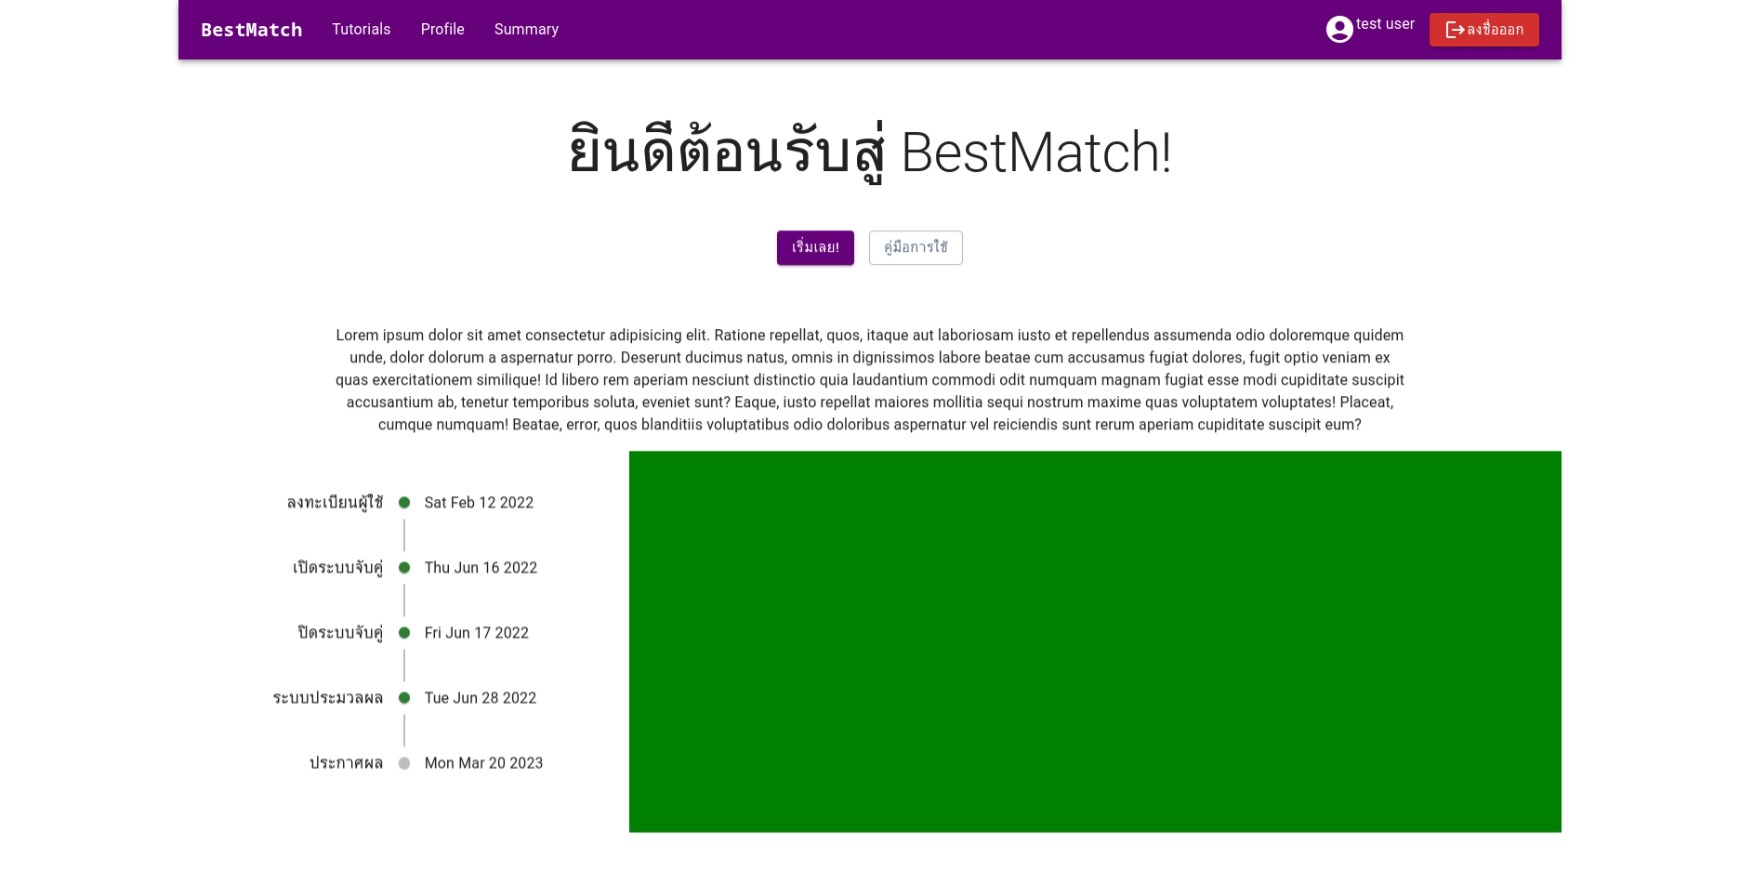
\includegraphics[width=\linewidth]{photo/web/student/home-auth.jpeg}
  \end{center}
  \caption{หน้า Home หลังยืนยันตัวตนสำเร็จ}
\end{figure}
%
\newline
เมื่อกดปุ่ม "เริ่มเลย" จะไปที่หน้าแอพพลิเคชันหลัก ซึ่งจะให้ผู้ใช้ระบุโปรไฟล์ของตนเอง
เสร็จแล้วกดปุ่ม "NEXT"
\begin{figure}[h]
  \begin{center}
    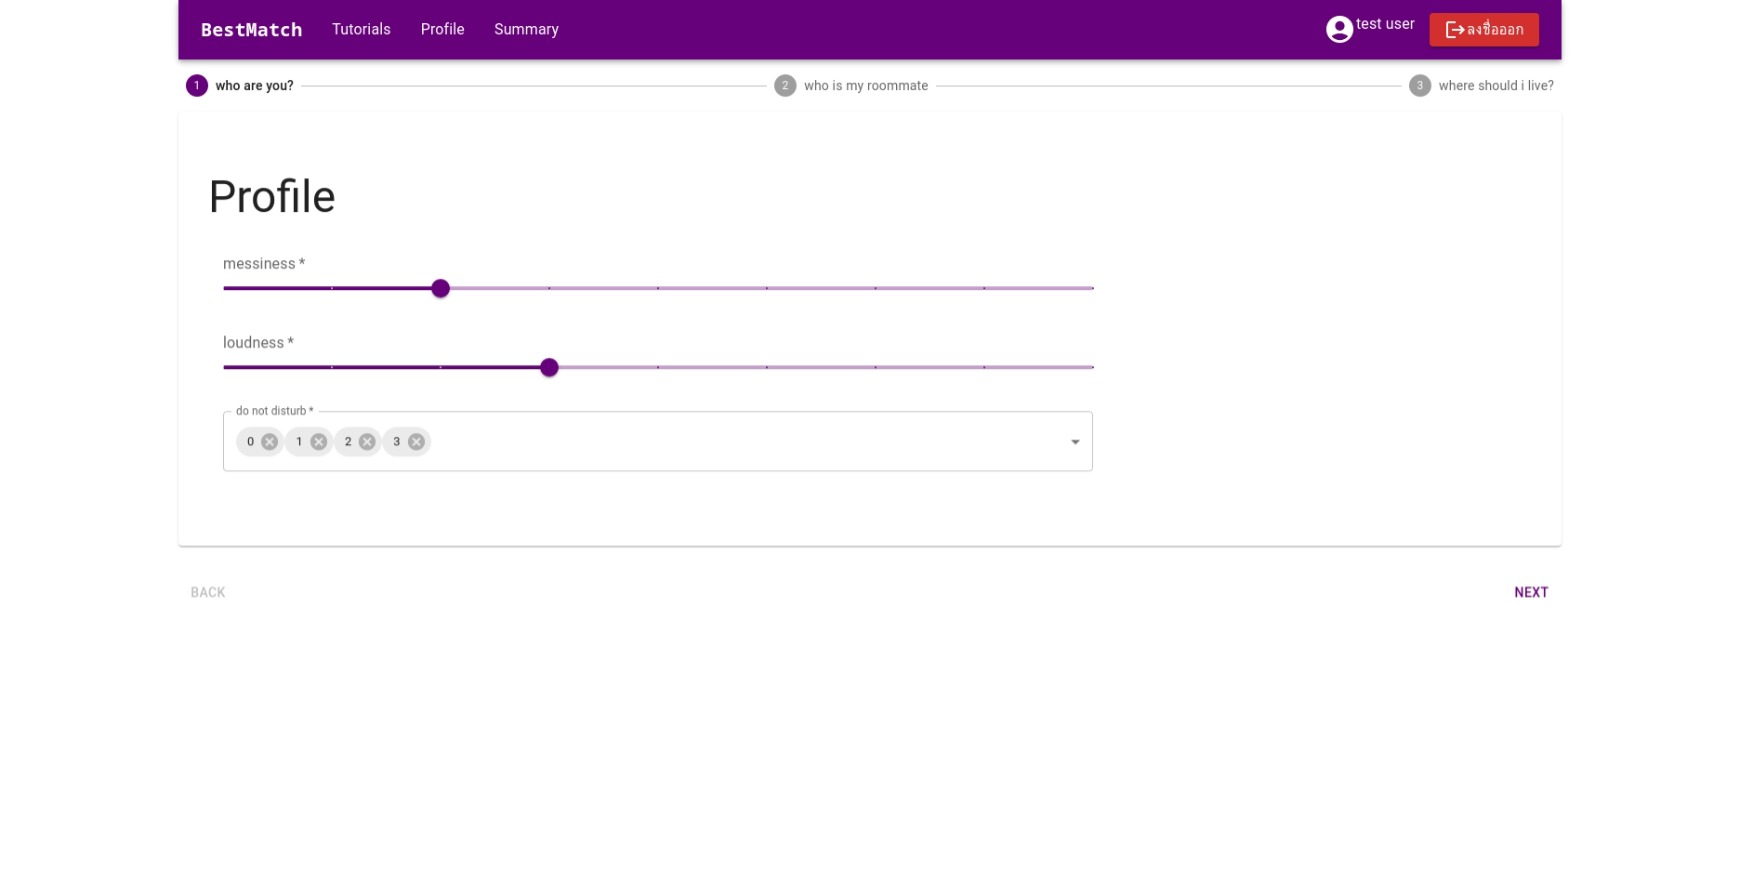
\includegraphics[width=\linewidth]{photo/web/student/profile-def.jpeg}
  \end{center}
  \caption{หน้าระบุ profile ของผู้ใช้}
\end{figure}
\newpage

หลังจากนั้นระบุ preference ของรูมเมทที่ต้องการ เมื่อเสร็จแล้วกดปุ่ม "NEXT"
\begin{figure}[h]
  \begin{center}
    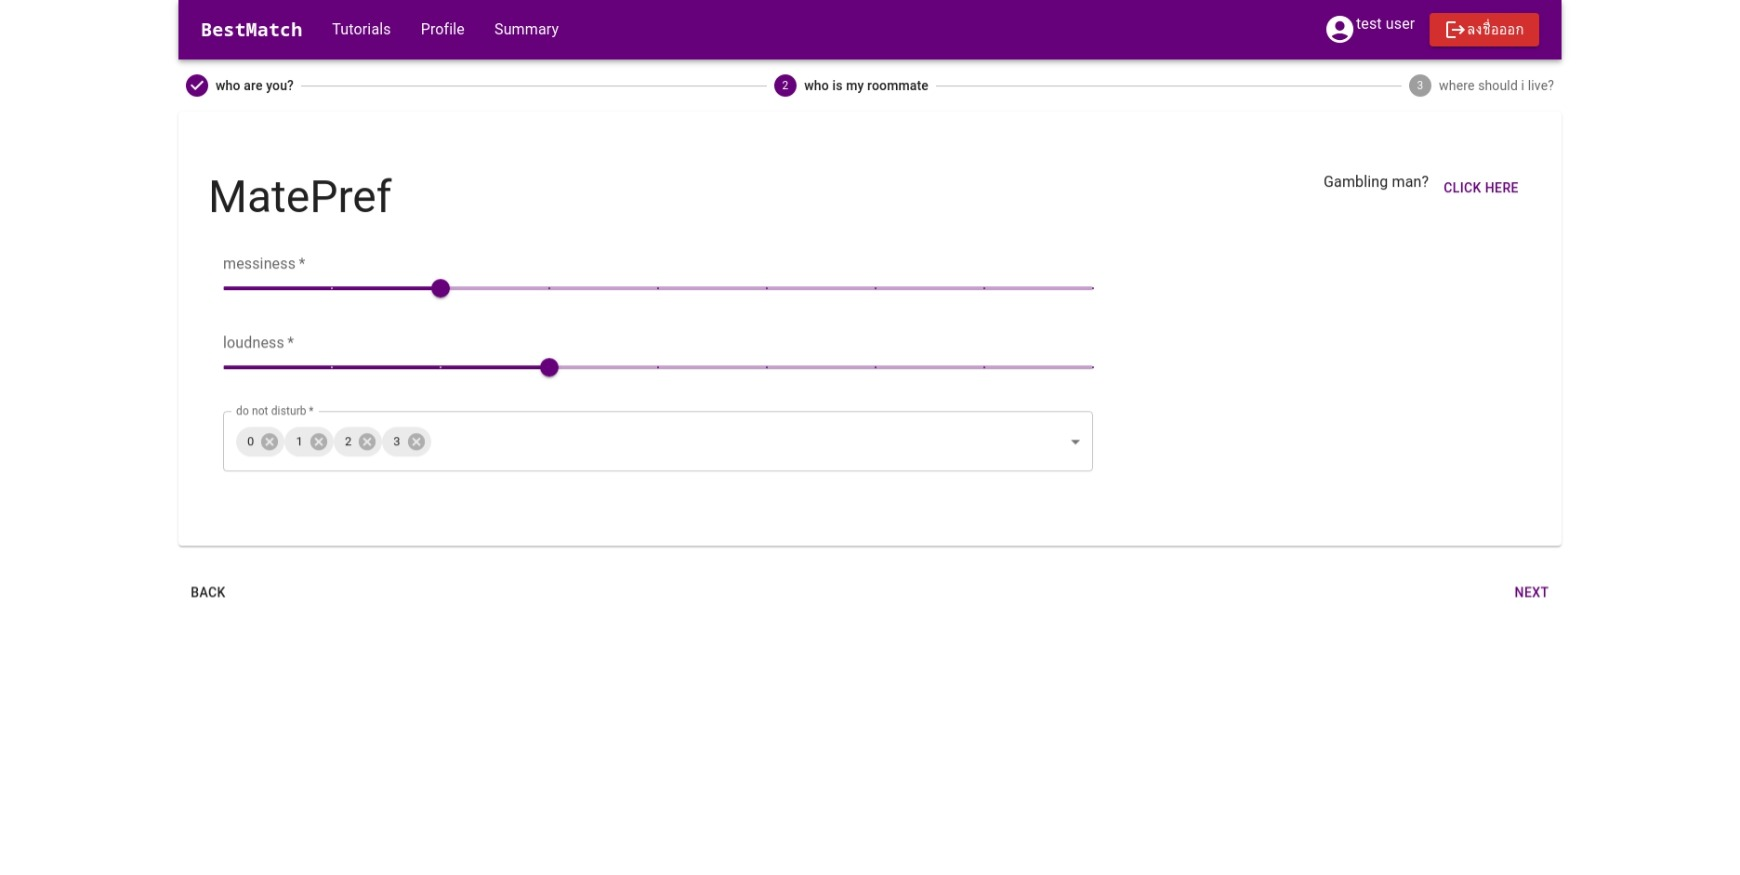
\includegraphics[width=\linewidth]{photo/web/student/mate-def.jpeg}
  \end{center}
  \caption{หน้า preference ของรูมเมท}
\end{figure}
%
\newline
โดยหากผู้ใช้ไม่อยากระบุ preference ของรูมเมทก็สามารถกด "CLICK HERE" ได้
\begin{figure}[h]
  \begin{center}
    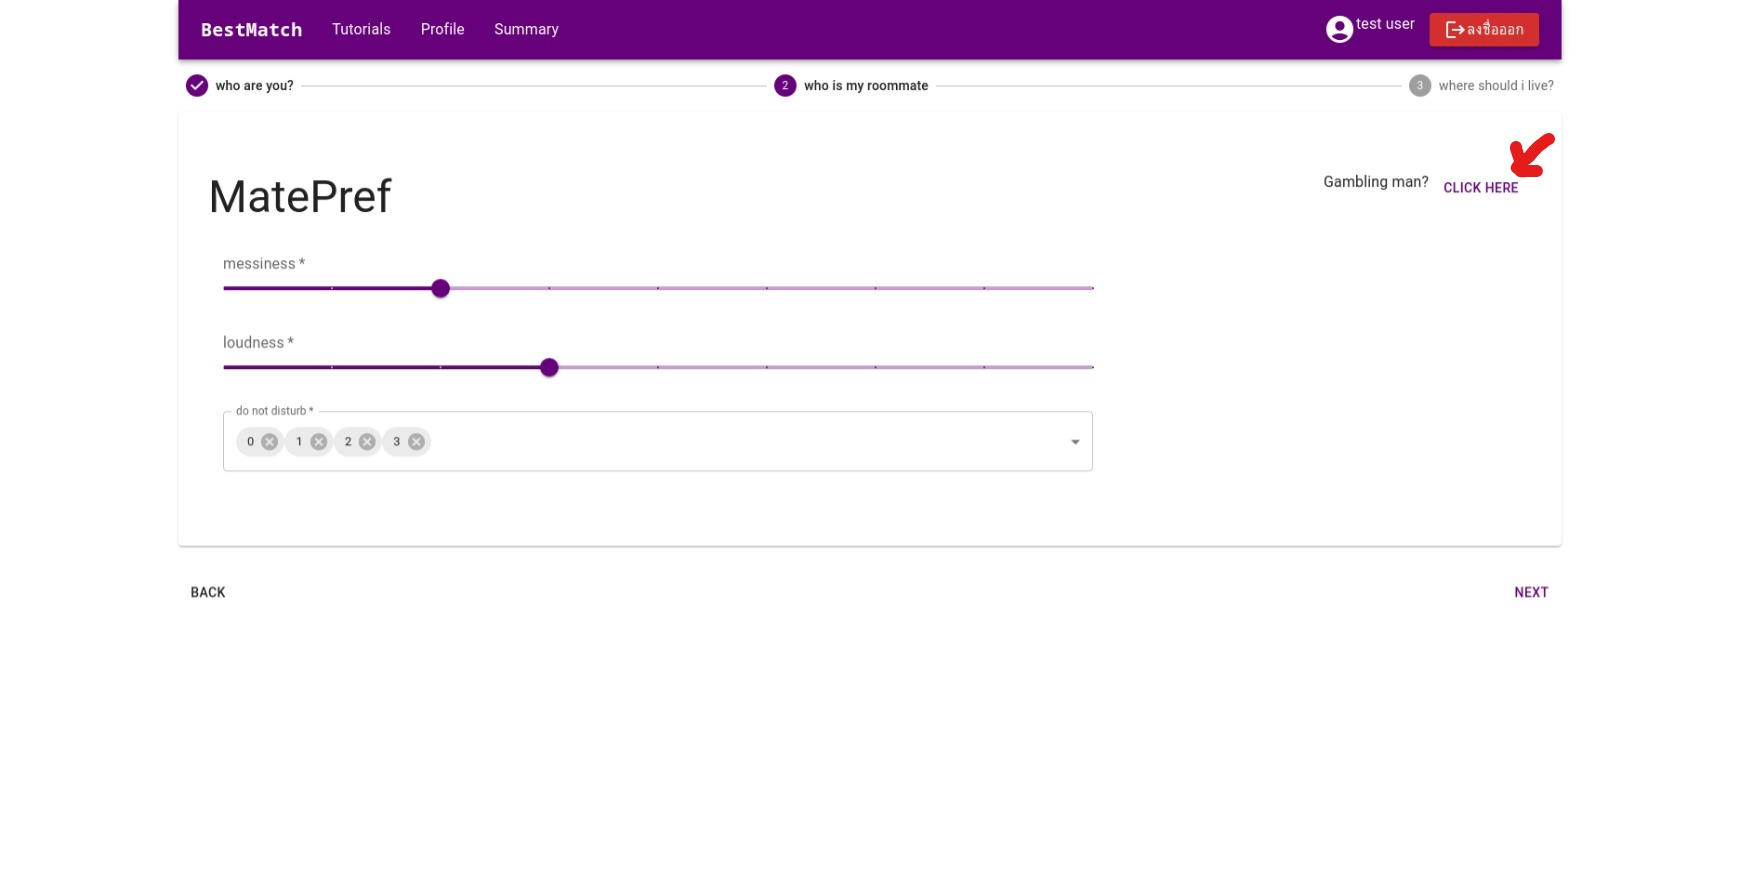
\includegraphics[width=\linewidth]{photo/web/student/mate-gambler.jpeg}
  \end{center}
  \caption{รูปตัวอย่างแสดงตำแหน่งปุ่ม "CLICK HERE" ของหน้า preference ของรูมเมท}
\end{figure}
\newpage

หลังจากนั้นระบุ preference ของห้อง และ หอพักที่ต้องการ เมื่อเสร็จแล้วกดปุ่ม "NEXT"
\begin{figure}[h]
  \begin{center}
    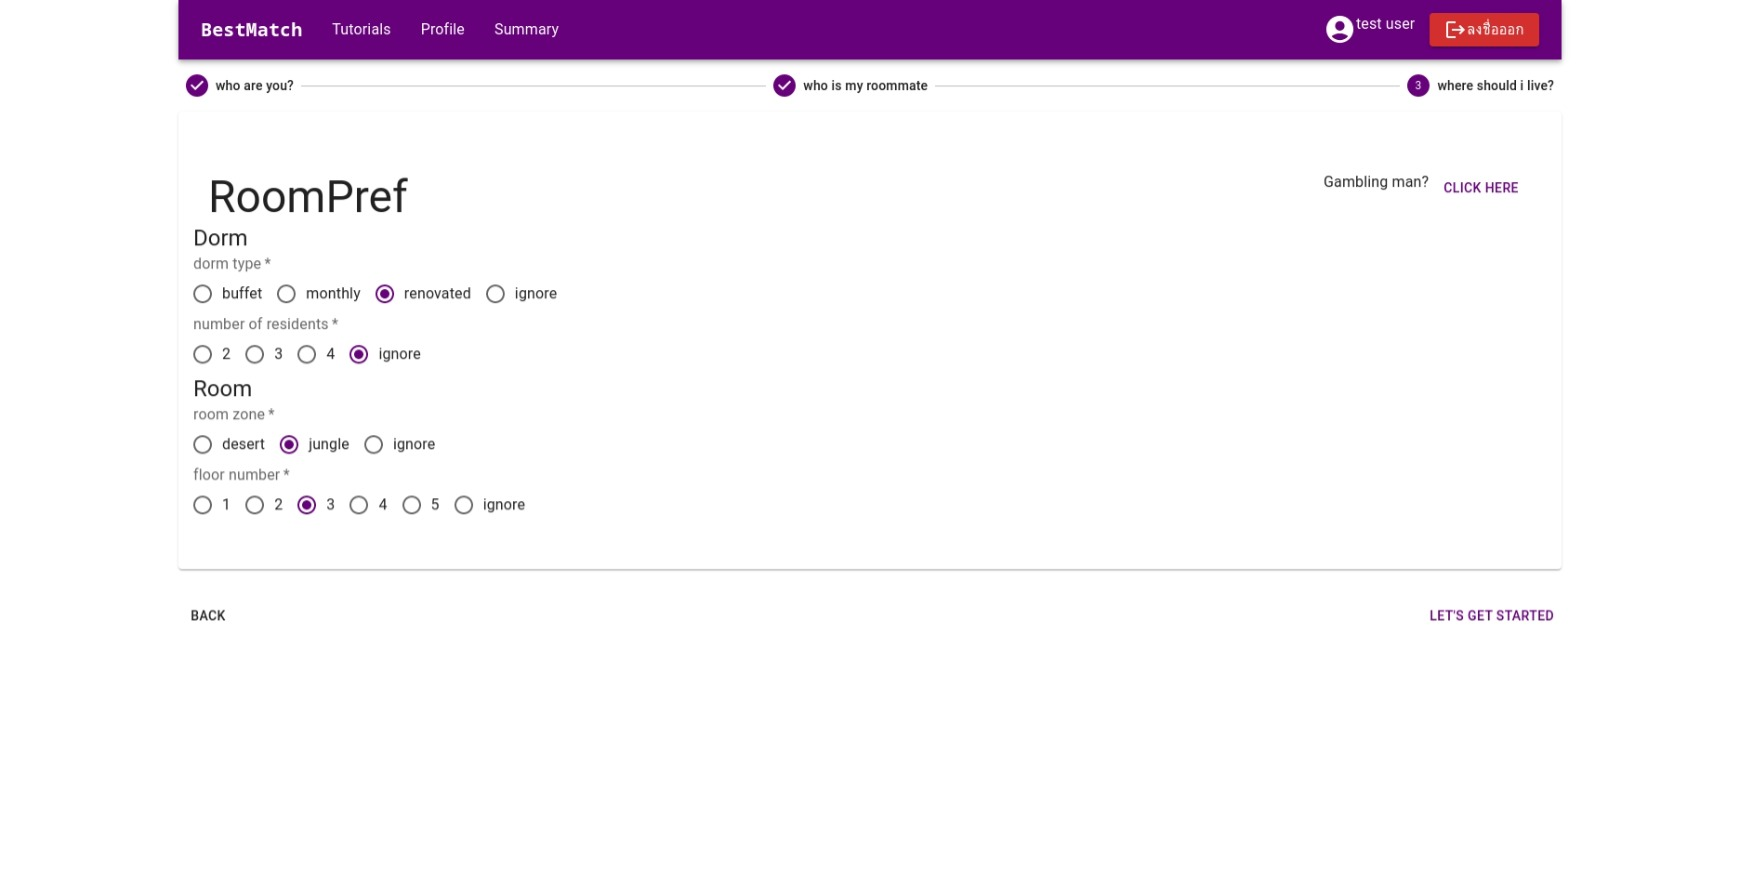
\includegraphics[width=\linewidth]{photo/web/student/dorm-def.jpeg}
  \end{center}
  \caption{หน้า preference ของหอพัก}
\end{figure}
%
\newline
โดยหากผู้ใช้ไม่อยากระบุ preference ของหอพัก และห้องพักก็สามารถกด "CLICK HERE" ได้
\begin{figure}[h]
  \begin{center}
    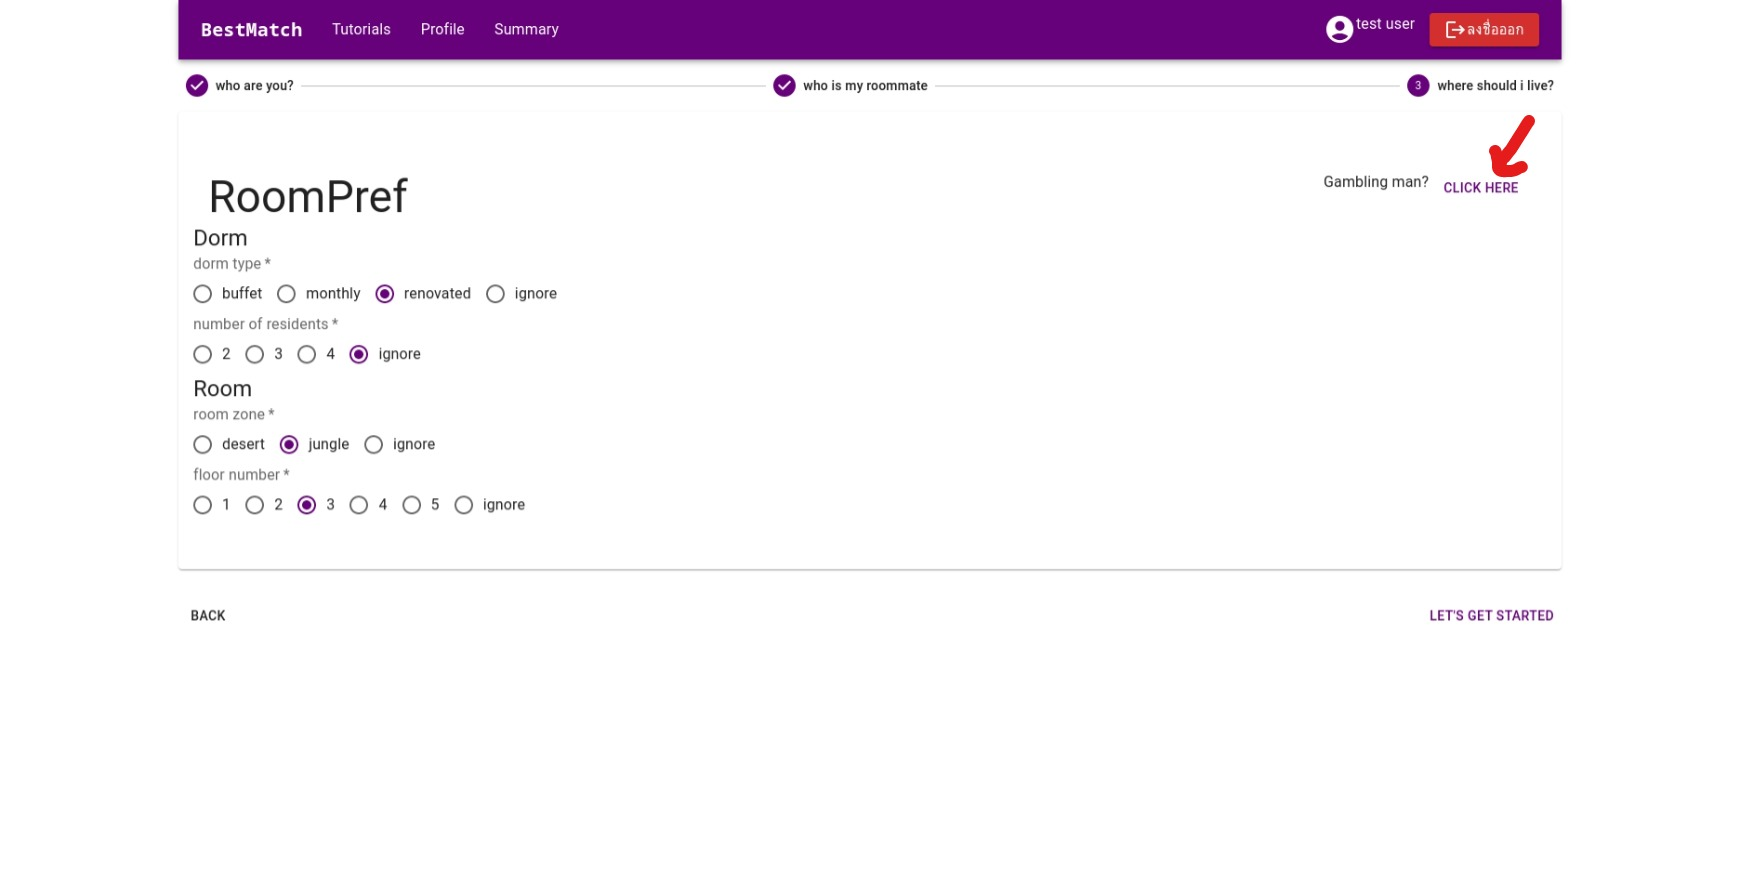
\includegraphics[width=\linewidth]{photo/web/student/dorm-gambler.jpeg}
  \end{center}
  \caption{รูปตัวอย่างแสดงตำแหน่งปุ่ม "CLICK HERE" ของหน้า preference ของหอพัก}
\end{figure}
\newpage

หลังจากนั้นจะเป็นหน้าที่ให้ผู้ใช้เลือกว่าจะเอาโปรไฟล์สมมุติ โปรไฟล์ไหนสำหรับการ finetune
\begin{figure}[ht]
  \begin{center}
    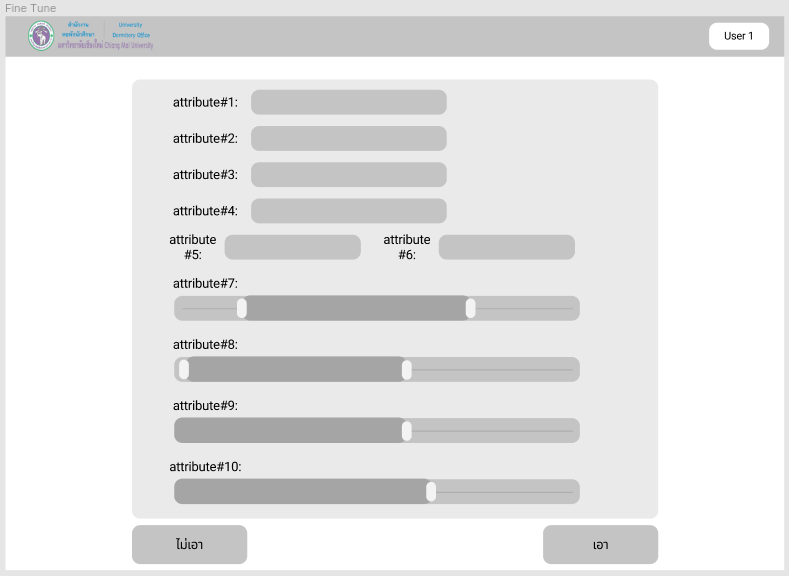
\includegraphics[width=\linewidth]{photo/web/student/finetune.jpeg}
  \end{center}
  \caption{หน้า Finetune}
\end{figure} 
%
\newline
หากผู้ใช้พึงพอใจกับการ finetune แล้วสามารถกลับหน้า Home ได้โดยคลิกที่ไอคอน "BESTMATCH"
\begin{figure}[ht]
  \begin{center}
    \includegraphics[width=\linewidth]{photo/web/student/finetune_home.jpeg}
  \end{center}
  \caption{รูปตัวอย่างแสดงตำแหน่งปุ่มไอคอน "BESTMATCH" เพื่อกลับไปที่หน้าหลัก}
\end{figure}
\newpage

ซึ่งผู้ใช้สามารถตรวจสอบโปรไฟล์ของตนเองได้ที่หน้า Profile
\begin{figure}[h]
  \begin{center}
    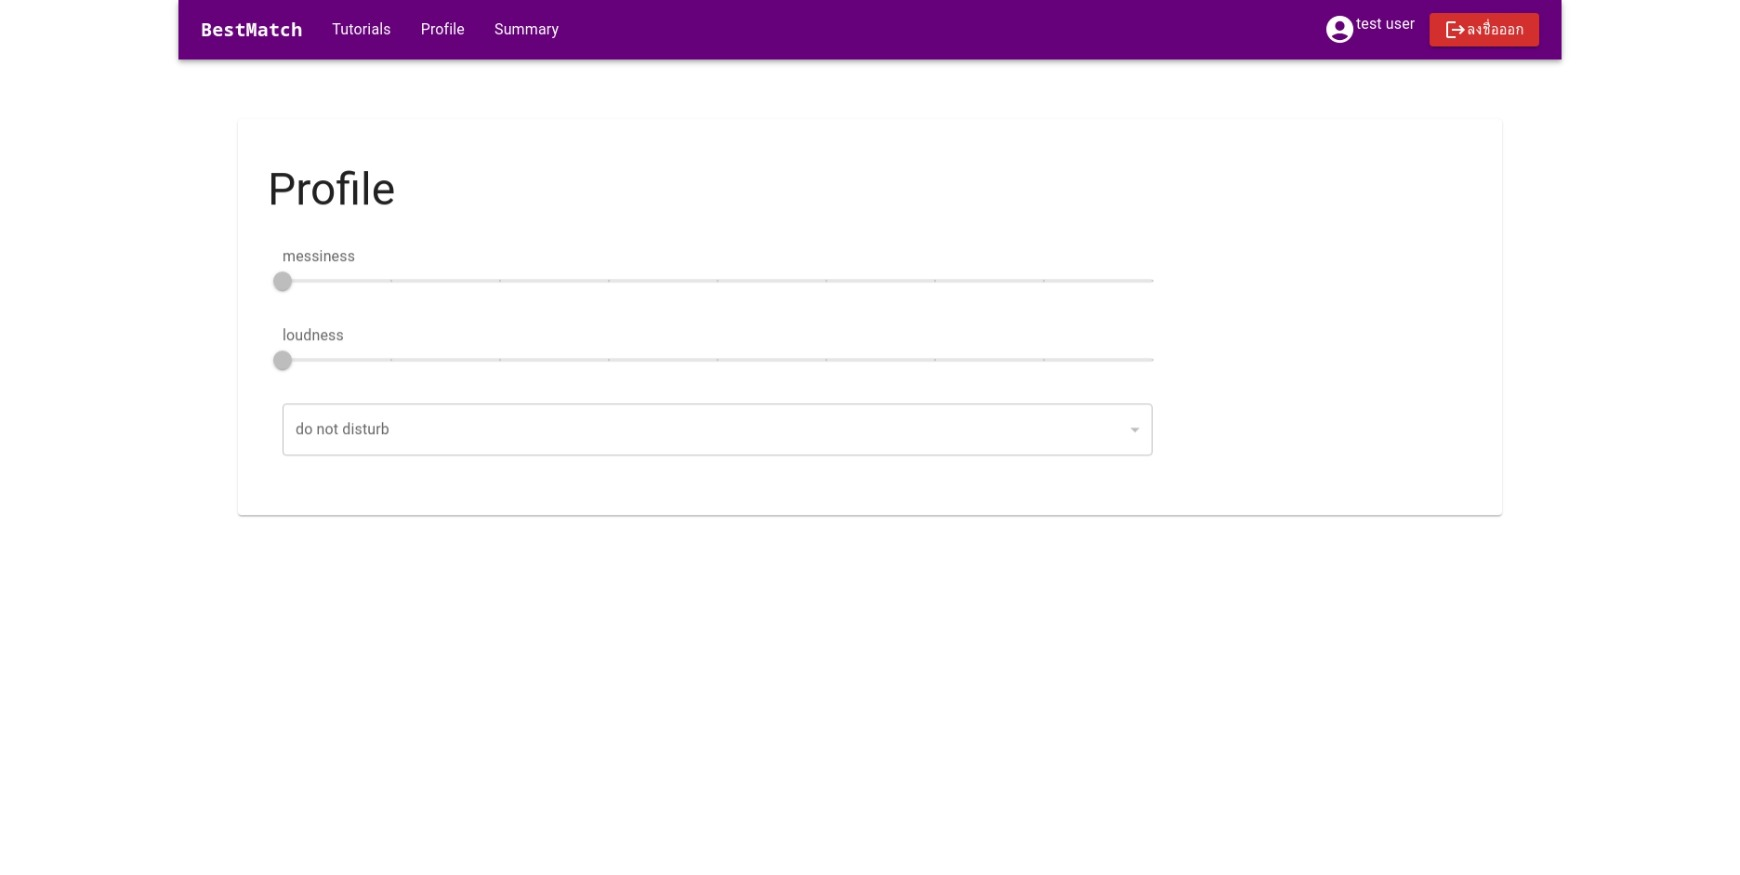
\includegraphics[width=\linewidth]{photo/web/student/profile.jpeg}
  \end{center}
  \caption{หน้า Profile}
\end{figure}
%
\newline
และสามารถตรวจสอบรูมเมทที่คาดว่าจะได้จากการจับคู่ที่หน้า Summary
\begin{figure}[h]
  \begin{center}
    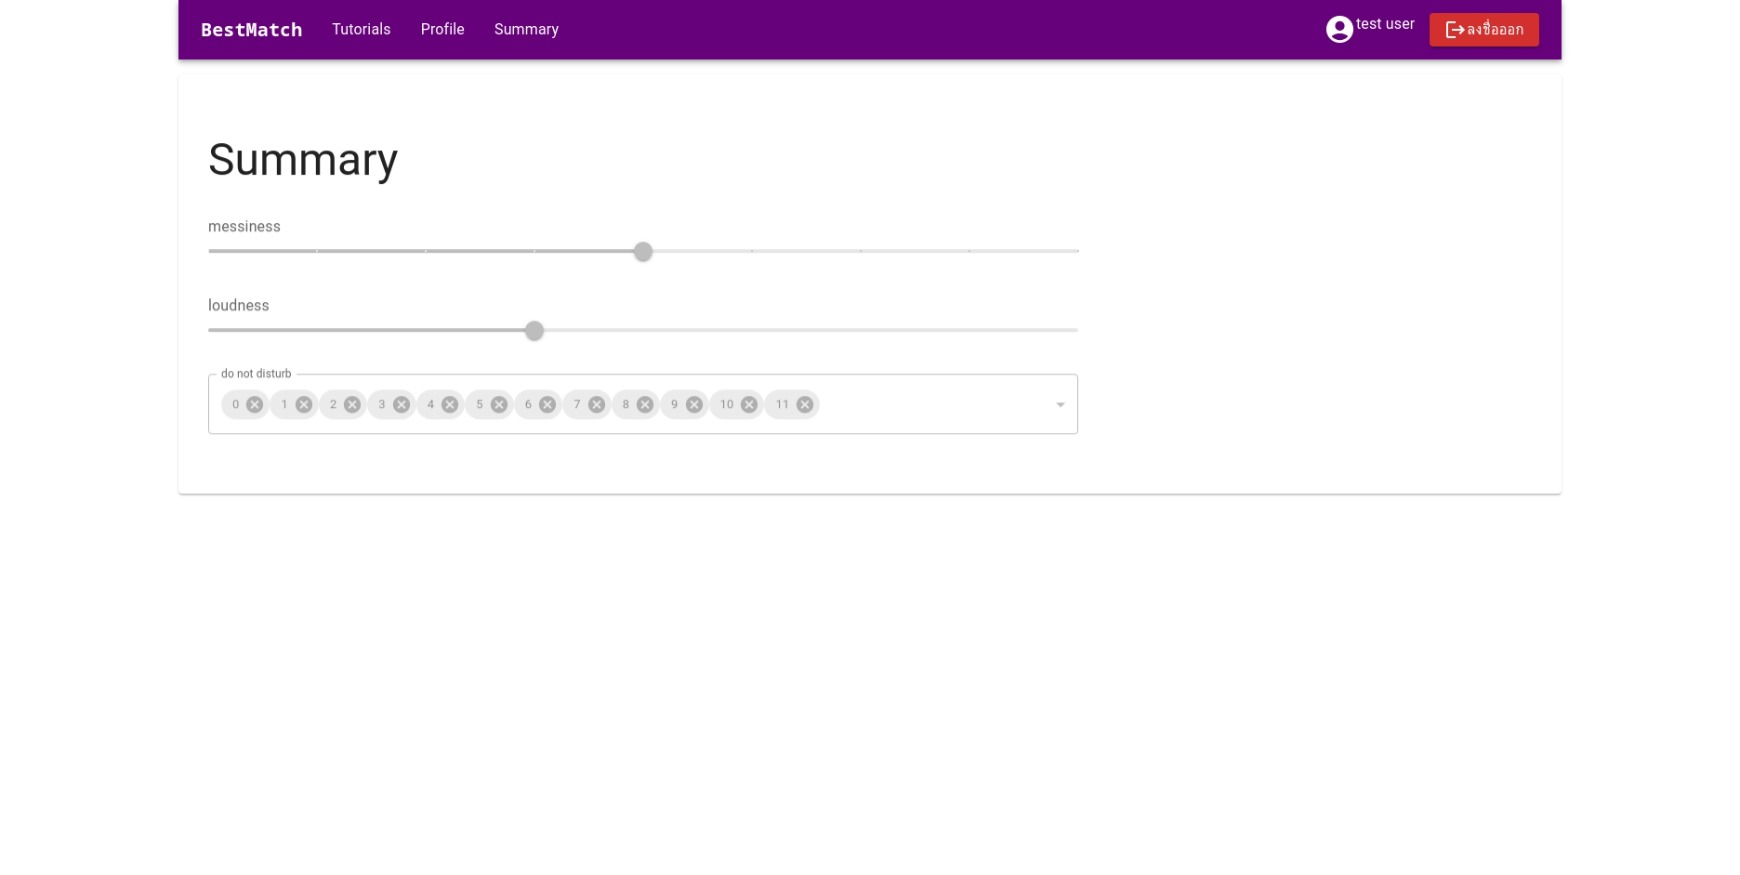
\includegraphics[width=\linewidth]{photo/web/student/summary.jpeg}
  \end{center}
  \caption{หน้า Summary}
\end{figure}